\chapter*{Breve Panoramica sul Protocollo CRTP}
\addcontentsline{toc}{chapter}{Breve Panoramica sul Protocollo CRTP}

Il protocollo CRTP (Crazy Real Time Protocol) è il protocollo creato appositamente da Bitcraze per gestire la comunicazione da/verso il Drone. 
\\
Concettualmente la comunicazione che avviene tra il Drone e la Crazyradio segue il seguente schema: 
\begin{figure}[h]
    \centering
    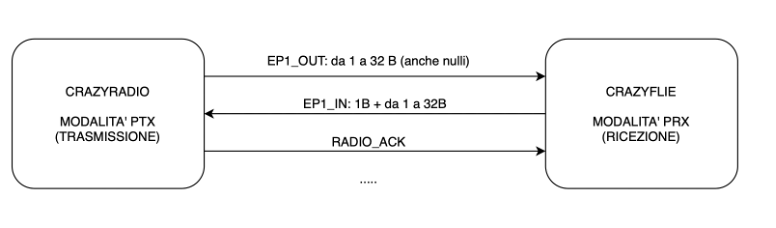
\includegraphics[width=0.8 \textwidth]{Relazione/Immagini/handshake.png}
    \caption{Handshake CRTP}
    \label{fig:Handshake}
\end{figure}
\\
Le relative implementazioni Python dei due blocchi sopra mostrati sono le seguenti: 

\begin{figure}[h]
    \centering
    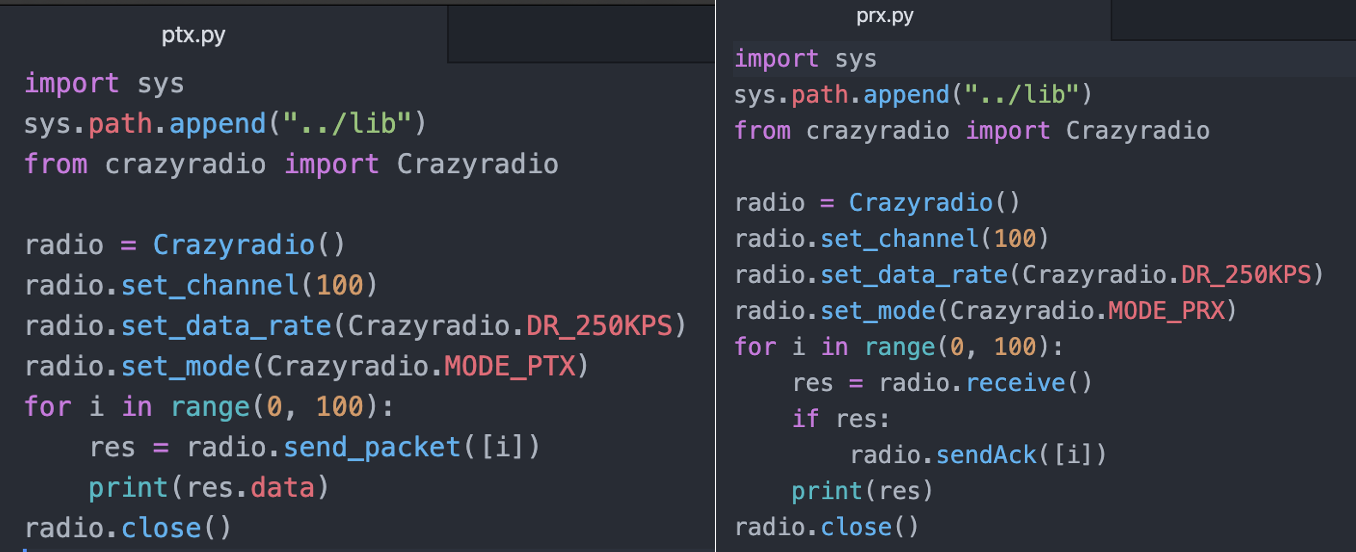
\includegraphics[width=0.8 \textwidth]{Relazione/Immagini/HandshakePython.png}
    \caption{Handshake CRTP con funzioni Python}
    \label{fig:HandshakePyhton}
\end{figure}
\\
Andando più nel dettaglio abbiamo visto come questo protocollo  si avvale di  pacchetti che hanno la seguente struttura: 
\\
\begin{figure}[h]
    \centering
    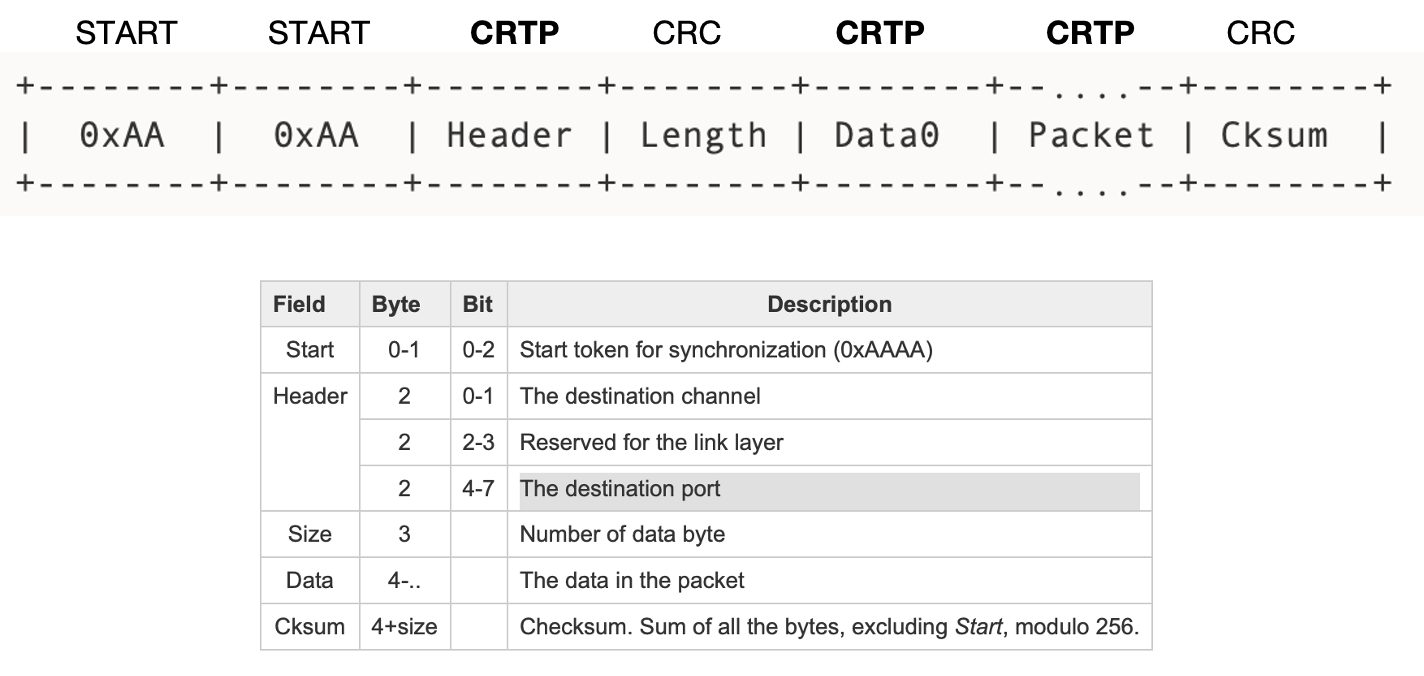
\includegraphics[width=0.8 \textwidth]{Relazione/Immagini/PacchettiCRTP.png}
    \caption{Pacchetti CRTP - Specifichiamo che il campo Data può contenere al massimo 31B}
    \label{fig:PacchettiCRTP}
\end{figure}
\\
Un’ulteriore analisi della codifica della Porta di destinazione è necessaria: \begin{figure}[h]
    \centering
    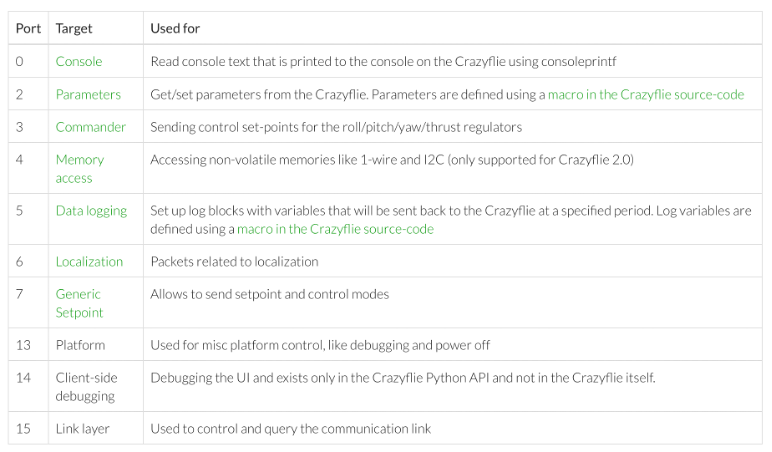
\includegraphics[width=0.8 \textwidth]{Relazione/Immagini/PorteDestinazione.png}
    \caption{Codifica porte di destinazione dei pacchetti CRTP}
    \label{fig:PorteDestinazione}
\end{figure}
\\
Di seguito riportiamo un banale esempio in cui vediamo come dovrebbe essere fatto un pacchetto per voler inviare al \verb Commander  (porta 3) un campo \verb Data  contenente riferimenti nulli di orientazione e spinta dei motori:
\begin{figure}[h]
    \centering
    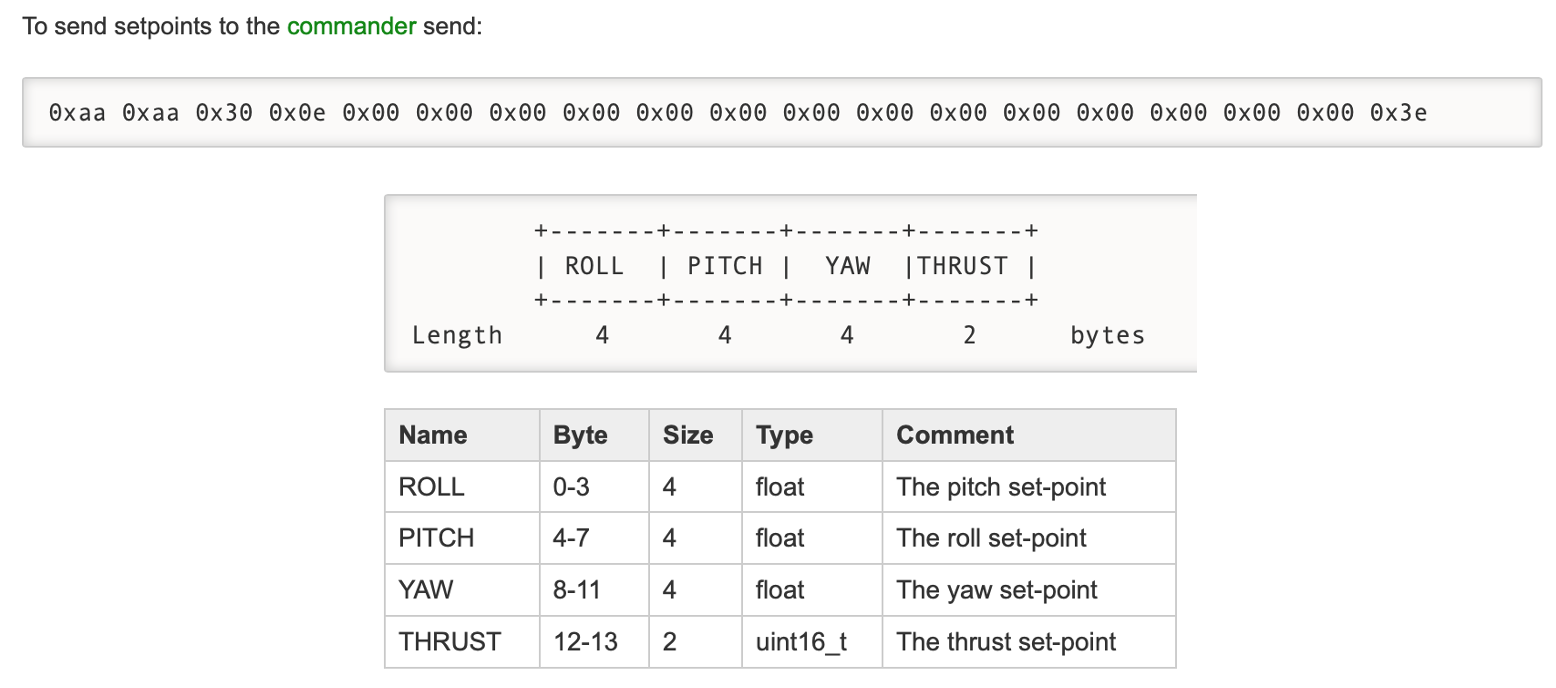
\includegraphics[width=0.9 \textwidth]{Relazione/Immagini/EsempioCommander.png}
    \caption{Esempio di invio pacchetto CRTP}
    \label{fig:EsempioCommander}
\end{figure}
\\
\\
\\
\\
\\
\\
\\
Tornando  allo scopo del progetto, è per noi di interesse la porta 6 utilizzata per la trasmissione di pacchetti contenenti informazioni di posizione e orientazione.  \\
Di seguito vediamo come, tramite la codifica di due diversi “canali”, possiamo utilizzare questa porta per la trasmissione di informazioni automaticamente indirizzate al filtro di Kalman (utilzzando il \textbf{canale 0}):
\begin{figure}[h]
    \centering
    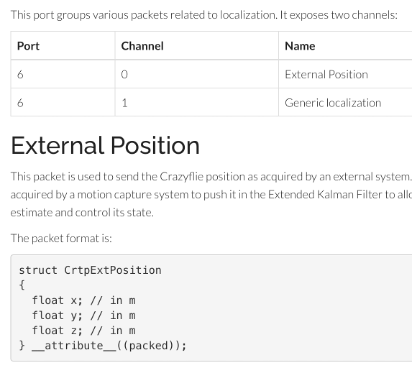
\includegraphics[width=0.6 \textwidth]{Relazione/Immagini/externalposition.png}
    \caption{External Position}
    \label{fig:externalposition}
\end{figure}
\\
\\


Qualora volessimo trasmettere anche l’informazione dell’orientazione, in aggiunta a quella di posizione, dobbiamo avvalerci del \textbf{canale 1} che consente l’invio di una struttura dati di dimensioni maggiori, come mostrato di seguito: 
\begin{figure}[h]
    \centering
    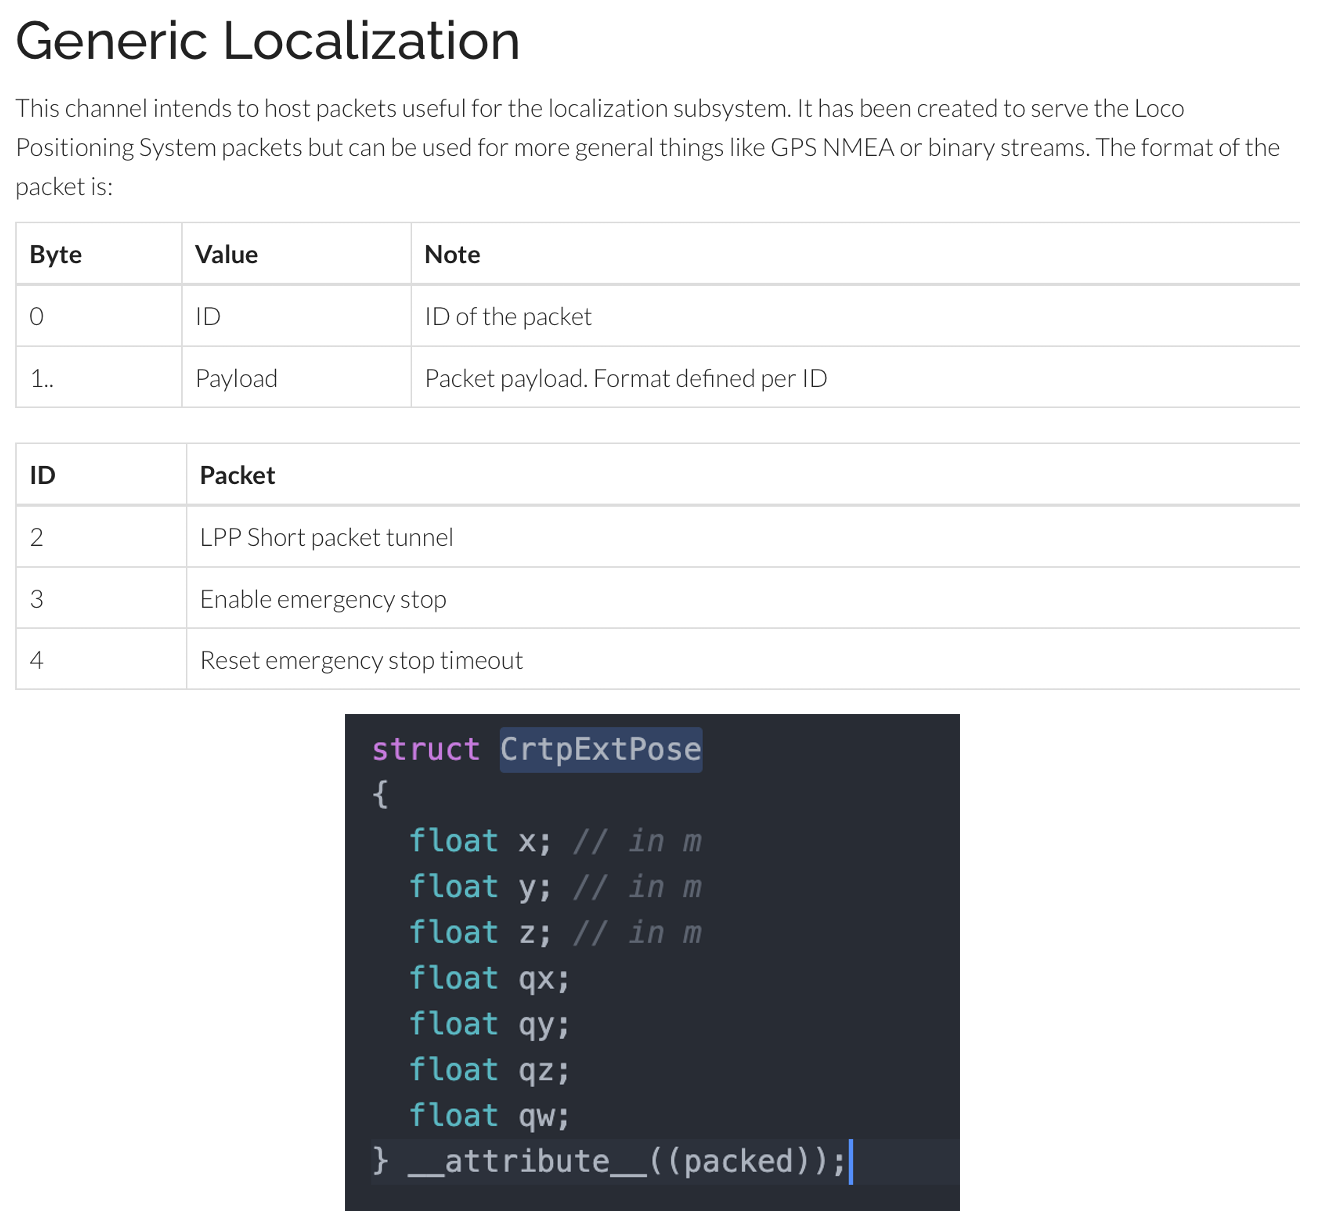
\includegraphics[width=0.8 \textwidth]{Relazione/Immagini/genericLocalization.png}
    \caption{External Position}
    \label{fig:genericLocalization}
\end{figure}

